\section{Checks concerning the enhancement at low \Dz\proton mass}
\label{sec:Structure}

In section \ref{sec:Signalfit} it has been stated that the fit of the \Dz\proton mass spectrum needs an additional component to parametrize an enhancement at low \Dz\proton masses right after threshold.
An appropriate model for that enhancement has seemed to be parametrized like the two \LcResI and \LcResII resonances.
This doesn't mean at all that there is really an additional resonance seen.
There might be a lot of other reasons, e.g.:
\begin{itemize}
    \item Detector threshold / acceptance effects,
    \item Low mass behaviour induced by some selection requirements,
    \item Feed-down from partially reconstructed decays,
    \item Threshold enhancement due to wide resonances below \Dz\proton mass threshold.
\end{itemize}
In this chapter several checks are done to either explain the origin of this enhancement or rule out some of the ideas.
It should be mentioned, that there won't be a final answer to that question.
If this was really something new, it would be really hard to prove it with a semileptonic decay channel.
There is currently another \lhcb analysis on the exclusive hadronic decay \decay{\Lb}{\Dz\proton\pim} running, seeing a similar enhancement at low \Dz\proton mass.
This channel enables to study the enhancement with more methods for instance with an amplitude analysis making it possible to tell more about it.

\subsection{Detector threshold / acceptance effect}
One possible explanation of the enhancement might be a simple threshold respectively acceptance effect of the detector or caused by the application of some selection requirements.
To clarify this possibility and estimate the effects of the detector and the selection requirements the simulation samples at generator level and at reconstruction level are used.
Figure \ref{fig:detector_cut_effect} shows the invariant \Dz\proton mass at different stages in generation and reconstruction.
The green distribution shows the \Dz\proton mass at generation level, i.e. there's no simulation of the detector or any reconstruction applied here.
In blue one sees the \Dz\proton mass after the simulation of the detector and in red the mass after reconstruction and selection.
For comparison the measured data distribution is shown in black as well.
In this case always the so called ``true" masses are plotted, i.e. there are no influences of the detector resolution in these distributions.
This figure shows that the distribution behaves similar and there isn't any significant acceptance effect arising neither due to the detector itself nor due to the reconstruction and selection process. 
Thus, the enhancement can't be caused by such an effect.
\begin{figure}[hptb]
	\centering
	\includegraphics[width=0.49\textwidth]{LbToD0p/structure/detector_cut_effect}
	\caption{Simulated (true) invariant \Dz\proton mass at different stages, namely after generation (green), detector simulation (blue) and reconstruction and selection (red). The black line shows the measured data.}
	\label{fig:detector_cut_effect}
\end{figure}

Excluded to get any structure from acceptance effects a closer look at the \Dz\proton mass threshold reveals some kind of an ``S-shaped" curvature in the ascending part.
This can be better seen with a zoom into this region as shown in figure \ref{fig:mD0p_zoom}.
\begin{figure}[hptb]
	\centering
	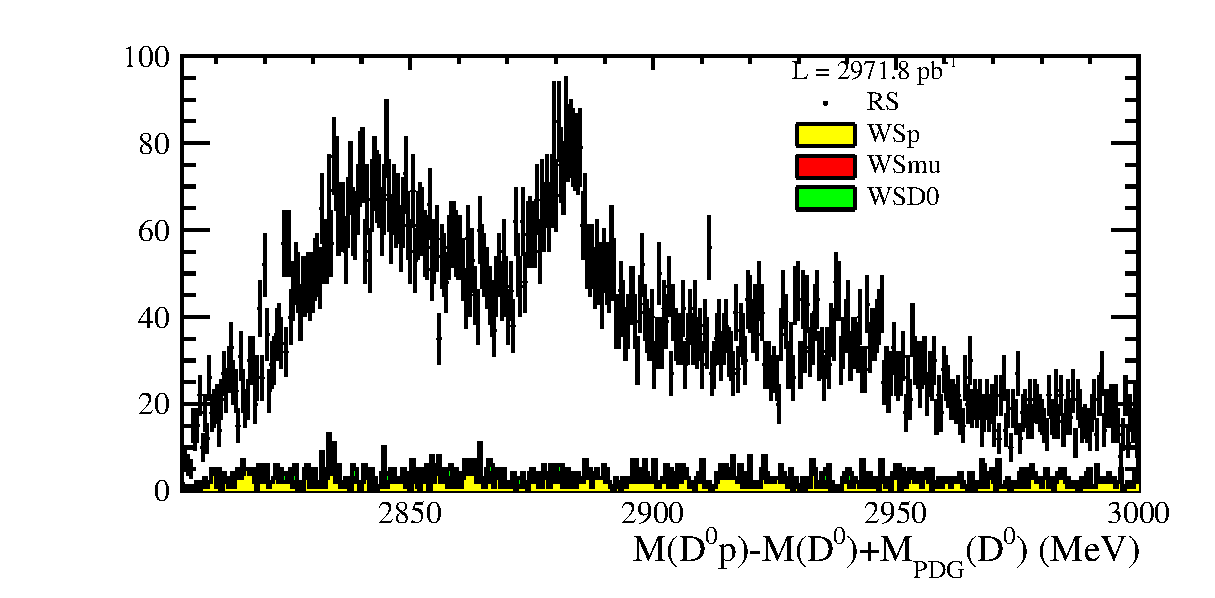
\includegraphics[width=0.49\textwidth]{LbToD0p/plots/data/Bh_DELTA_MASS_zoom}
	\caption{Zoom into the low \Dz\proton mass region.}
	\label{fig:mD0p_zoom}
\end{figure}

Due to this curvature the fit isn't able to describe the low \Dz\proton mass region only with a nonresonant component but rather prefers to have an additional component. 
At this point it should be mentioned that there are other analyses seeing a similar behaviour in this \Dz\proton mass region.

First of all, there is a study by \babar on the \Dz\proton final state (see fig. \ref{fig:Babar_D0p} aiming to measure the \LcResI and \LcResII resonance (and in the latter case to even observe it).
While discussing their systematics, they're wondering if this much less pronounced (compared to this analysis) bump at roughly 2840\mev might change their results by adding an additional resonance component to their fit. 
Since the impact isn't that large they just include the deviations in their systematics, unfortunately without trying to understand the origin of this bump \cite{Babar_D0p}.
\begin{figure}[hptb]
	\centering
	\includegraphics[width=0.49\textwidth]{Babar_D0p}
	\caption{\babar study on the \Dz\proton final state. They suspect to see a structure similar to the enhancement in the current analysis and fit it in c) with an additional resonance component for their systematic studies. Figure taken from \cite{Babar_D0p}.}
	\label{fig:Babar_D0p}
\end{figure}

Furthermore, there are two more running \lhcb studies on either prompt \Dz\proton events and on the hadronic \decay{\Lb}{\Dz\proton\pim} decay.
It can be disclosed that they are struggling with the same problem, seeing a pronounced enhancement around 2840\mev without being (currently) able to explain it.
However, since there doesn't exist any approved material, nothing of their plots can be shown in this thesis.

Being seen in different channels and analysis substantiates the assumption, that there is a physical reason for the enhancement.

\subsection{Threshold enhancement from other resonances}


\subsection{Further ideas}
\begin{itemize}
    \item The unknown structure in the low mass region of the \Dz\proton spectrum could have its origin in the decay \decay{\SigmacpRes{(2880)}}{\Dz\proton}, which is kinematically exactly at threshold ($M(\proton)+M(\Dz)=2802\mev$).  
          The \SigmacpRes{(2880)} in turn could be part of the decay \decay{\SigmabpRes}{\SigmacpRes{(2880)}\mun\neumb}. 
          Another possibility would be \decay{\Lb}{\SigmacpRes{(2880)}\mun\neumb} which should be allowed by Feynman rules but might be forbidden by isospin violation since $I(\Lb) = 0$ and $I(\SigmacpRes{(2880)}) = 1$. 
          On the other hand weak decays don't respect isospin conservation.
          However, this resonance should lead to a threshold enhancement causing a steep smooth ascent at mass threshold and not having this ``S-curvature"
    \item The peak could come from a resonance decaying into an excited \Dstar(2007)\proton with \Dstar(2007) \to \Dz\pion where the \pion isn't reconstructed.
          The \LcResI is too light to decay in \Dstar(2007)\proton and even the \LcResII is slightly below the \Dstar(2007)\proton mass threshold of 2945 \mev. 
          Maybe there is a heavier resonance proceeding via this decay, maybe a partially reconstructed decay of a \Sigmacp.
    \item Direct product of an excited \Lc or \Sigmacp state. The muon should then randomly combined???
    \item 
    \item ...
\end{itemize}


